\documentclass[11pt]{article}

% ---------------------------------------------------------------------------
% BFL user decision guide --- how run_BFL() infers the variant from your inputs.
% Compiles on Overleaf (pdfLaTeX).
% ---------------------------------------------------------------------------
\usepackage[margin=0.9in]{geometry}
\usepackage{amsmath}
\usepackage{xcolor}
\usepackage{booktabs}
\usepackage{tabularx}
\usepackage{makecell}
\usepackage{enumitem}
\usepackage{listings}
\usepackage{tcolorbox}
\usepackage{hyperref}
\usepackage{tikz}
\usetikzlibrary{shapes.geometric, arrows.meta, positioning, calc}

\hypersetup{colorlinks=true, linkcolor=blue!50!black, urlcolor=blue!50!black}
\setlist{itemsep=1pt, topsep=2pt, parsep=0pt}
\newcolumntype{Y}{>{\raggedright\arraybackslash}X}

\definecolor{cIn}{HTML}{E8F0FE}
\definecolor{cProc}{HTML}{F1F3F4}
\definecolor{cDec}{HTML}{FEF7E0}
\definecolor{cBase}{HTML}{E6F4EA}
\definecolor{cDom}{HTML}{FCE8E6}
\definecolor{cPar}{HTML}{E8EAF6}
\definecolor{cCode}{HTML}{F6F8FA}

\tikzstyle{io}    = [rectangle, rounded corners, draw=black!60, fill=cIn, text width=6.4cm, align=center, minimum height=0.8cm, font=\scriptsize]
\tikzstyle{proc}  = [rectangle, draw=black!60, fill=cProc, text width=6.4cm, align=center, minimum height=0.7cm, font=\scriptsize]
\tikzstyle{dec}   = [diamond, aspect=2.3, draw=black!60, fill=cDec, text width=2.9cm, align=center, inner sep=1pt, font=\scriptsize]
\tikzstyle{term}  = [rectangle, rounded corners, draw=black!60, text width=3.7cm, align=center, minimum height=0.9cm, font=\scriptsize]
\tikzstyle{arrow} = [thick, -{Stealth[length=2mm]}]

\lstdefinestyle{R}{
  basicstyle=\ttfamily\footnotesize, backgroundcolor=\color{cCode},
  frame=single, rulecolor=\color{black!20}, breaklines=true,
  commentstyle=\color{green!45!black}, showstringspaces=false,
  language=R, columns=fullflexible, xleftmargin=4pt, framexleftmargin=4pt}

\newtcolorbox{notebox}[1]{colback=#1!8, colframe=#1!55!black, boxrule=0.6pt,
  arc=2pt, left=5pt, right=5pt, top=3pt, bottom=3pt}

\title{\vspace{-1.2em}\textbf{BFL: A User's Decision Guide}\\[2pt]
\large How \texttt{run\_BFL()} picks the model from \emph{how you build your inputs}}
\author{}\date{}

\begin{document}
\maketitle
\vspace{-3em}

% ===========================================================================
\section{Setup and notation}
A \textbf{target} site \textbf{T} (the one we want cause fractions for) and three
fully labeled \textbf{source} sites \textbf{A}, \textbf{B}, \textbf{C}. T is only
\emph{partly} labeled (say $20\%$ labeled, $80\%$ unlabeled).

\begin{center}
\renewcommand{\arraystretch}{1.2}
\begin{tabularx}{\textwidth}{@{}>{\bfseries}l Y@{}}
\toprule
Symbol & Meaning\\
\midrule
T; A, B, C        & target site; three fully labeled source sites\\
$T_X,\,T_Y$       & target feature matrix / cause labels\\
$A_X,\dots,C_Y$   & source feature matrices / cause labels\\
labeled rows      & the small labeled part of T\\
unlabeled rows    & the rest of T --- \textbf{we always score here}\\
T self-site       & a model trained on T's \emph{labeled} rows\\
\bottomrule
\end{tabularx}
\end{center}

\begin{itemize}
  \item \texttt{run\_BFL()} has \textbf{no} ``model type'' argument --- it
        \emph{infers} the variant from the shape of your inputs.
  \item The hinge: do your \texttt{local\_summaries} cover \emph{all} target
        rows or only the \emph{unlabeled} ones, and did you pass \texttt{Y\_target}?
  \item Every variant is \textbf{scored on the unlabeled rows}; the variants
        differ in what extra information they feed the model.
\end{itemize}

% ===========================================================================
\section{Stage 0 --- one-time setup (before any variant logic)}
\begin{enumerate}[label=\arabic*., leftmargin=1.6em]
  \item \texttt{X\_target} $\rightarrow$ numeric matrix.
  \item \texttt{n\_total} $\leftarrow$ number of rows of \texttt{X\_target}.
  \item \texttt{ref\_hashes} $\leftarrow$ one fingerprint per target row.
  \item \texttt{n\_stan} $\leftarrow$ number of rows your
        \texttt{local\_summaries} cover.
\end{enumerate}
\noindent The comparison \texttt{n\_stan} vs.\ \texttt{n\_total} drives the
whole decision.

% ===========================================================================
\section{The decision tree}
\begin{center}
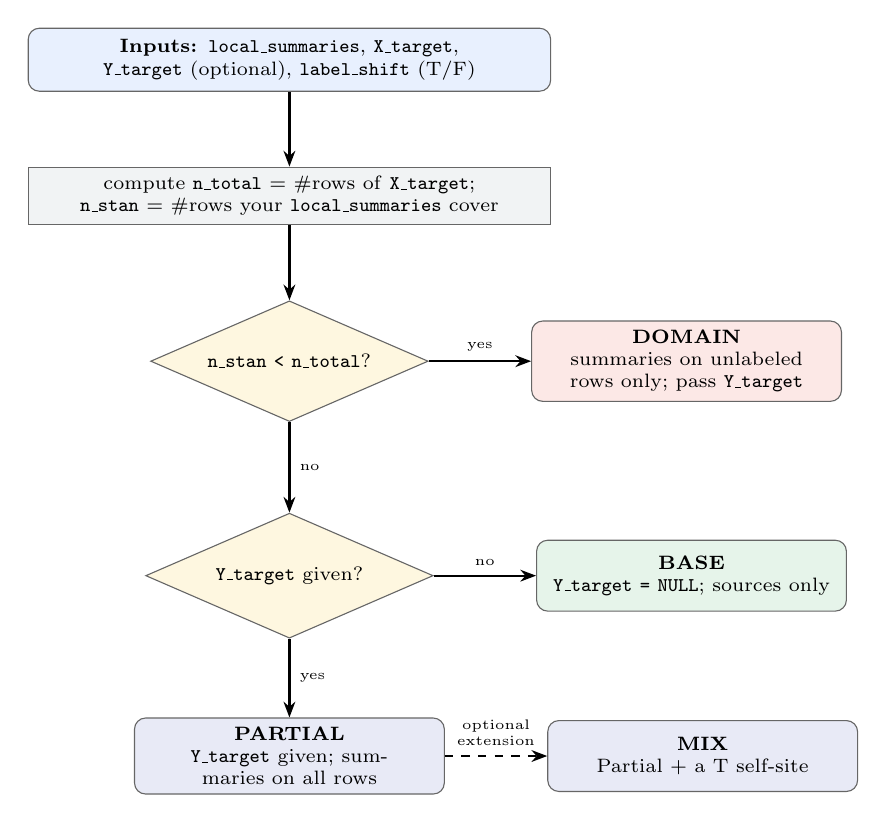
\begin{tikzpicture}[node distance=0.95cm and 1.1cm]
\node (start) [io] {\textbf{Inputs:} \texttt{local\_summaries}, \texttt{X\_target},
  \texttt{Y\_target} (optional), \texttt{label\_shift} (T/F)};
\node (setup) [proc, below=of start] {compute \texttt{n\_total} = \#rows of \texttt{X\_target}; \;\texttt{n\_stan} = \#rows your \texttt{local\_summaries} cover};
\node (decA) [dec, below=of setup] {\texttt{n\_stan < n\_total}?};
\node (domain) [term, fill=cDom, right=1.3cm of decA]
  {\textbf{DOMAIN}\\ summaries on unlabeled rows only; pass \texttt{Y\_target}};
\node (decB) [dec, below=1.15cm of decA] {\texttt{Y\_target} given?};
\node (base) [term, fill=cBase, right=1.3cm of decB]
  {\textbf{BASE}\\ \texttt{Y\_target = NULL}; sources only};
\node (partial) [term, fill=cPar, below=1.0cm of decB]
  {\textbf{PARTIAL}\\ \texttt{Y\_target} given; summaries on all rows};
\node (mix) [term, fill=cPar, right=1.3cm of partial]
  {\textbf{MIX}\\ Partial + a T self-site};

\draw [arrow] (start) -- (setup);
\draw [arrow] (setup) -- (decA);
\draw [arrow] (decA) -- node[above,font=\tiny]{yes} (domain);
\draw [arrow] (decA) -- node[right,font=\tiny]{no} (decB);
\draw [arrow] (decB) -- node[above,font=\tiny]{no} (base);
\draw [arrow] (decB) -- node[right,font=\tiny]{yes} (partial);
\draw [arrow, dashed] (partial) -- node[above,font=\tiny,align=center]{optional\\ extension} (mix);
\end{tikzpicture}
\end{center}

\begin{notebox}{orange}
\textbf{\texttt{label\_shift} (T/F) --- set on every run; chooses the CSMF target.}
\begin{itemize}
  \item \texttt{FALSE}: score against the \emph{whole} target. When labels enter
        Stan (Partial/Mix) the \texttt{balanced} model is used; Domain folds the
        known labeled counts $n_{Lc}$ back in.
  \item \texttt{TRUE}: score against the \emph{unlabeled rows only}; Partial/Mix
        use the \texttt{unbalanced} model.
\end{itemize}
\textbf{Base} is unaffected --- no labels reach Stan, so it is always
\texttt{no\_partial}, scored on the whole target.
\end{notebox}

\vspace{3pt}
\begin{notebox}{red}
\textbf{Domain check:} summaries must cover \emph{exactly} the unlabeled rows
(\texttt{\#NA(Y\_target) == n\_stan}), else \texttt{run\_BFL} errors.
\end{notebox}

\vspace{2pt}
\noindent\textbf{Partial vs.\ Mix is not a branch.} \texttt{run\_BFL} can't tell
them apart --- \textbf{Mix is just Partial with one extra model} (a T self-site)
added to \texttt{local\_summaries}.

% ===========================================================================
\section{Building \texttt{local\_summaries}}
\label{sec:build}
Each entry is one model's per-record scores (\texttt{posterior\_phi},
\texttt{cause\_ids}, \texttt{row\_hash}). ``T self-site'' = an LCVA trained on
T's \emph{labeled} rows, then used to produce phi.

\begin{center}
\renewcommand{\arraystretch}{1.2}
\setlength{\tabcolsep}{11pt}
\begin{tabular}{@{}lllll@{}}
\toprule
\textbf{Variant} & \makecell[l]{\textbf{Models in}\\\textbf{\texttt{local\_summaries}}}
 & \makecell[l]{\textbf{Summaries on}\\\textbf{target rows}}
 & \makecell[l]{\textbf{Predict /}\\\textbf{score on}} & \textbf{\texttt{Y\_target}}\\
\midrule
Base    & \makecell[l]{sources\\A, B, C}               & all rows       & unlabeled rows & \texttt{NULL}\\
\addlinespace
Domain  & \makecell[l]{sources A, B, C\\+ T self-site}  & unlabeled only & unlabeled rows & \makecell[l]{labels\\(\texttt{NA} on unlab.)}\\
\addlinespace
Partial & \makecell[l]{sources\\A, B, C}               & all rows       & unlabeled rows & \makecell[l]{labels\\(\texttt{NA} on unlab.)}\\
\addlinespace
Mix     & \makecell[l]{sources A, B, C\\+ T self-site}  & all rows       & unlabeled rows & \makecell[l]{labels\\(\texttt{NA} on unlab.)}\\
\bottomrule
\end{tabular}
\end{center}

\subsection*{Base --- sources only, no labels}
\begin{lstlisting}[style=R]
ls <- list(A = sumA, B = sumB, C = sumC)        # phi on ALL target rows
run_BFL(ls, X_target = T_X, Y_target = NULL, label_shift = FALSE)
\end{lstlisting}

\subsection*{Domain --- sources + T self-site, on the unlabeled rows}
\begin{lstlisting}[style=R]
selfFit <- LCVA.train(X = T_X_lab, Y = T_Y_lab)      # T's labeled rows
sumT    <- summarise(predict_phi(selfFit, T_X_unlab))# phi on unlabeled rows
ls <- list(A = sumA_unlab, B = sumB_unlab, C = sumC_unlab, T = sumT)
Y  <- T_Y; Y[unlabeled] <- NA
run_BFL(ls, X_target = T_X, Y_target = Y, label_shift = FALSE)
\end{lstlisting}

\subsection*{Partial --- sources only, labels fed to the model}
\begin{lstlisting}[style=R]
ls <- list(A = sumA, B = sumB, C = sumC)        # phi on ALL rows
Y  <- T_Y; Y[unlabeled] <- NA
run_BFL(ls, X_target = T_X, Y_target = Y, label_shift = FALSE)
\end{lstlisting}

\subsection*{Mix --- Partial \emph{plus} a T self-site (the only change)}
\begin{lstlisting}[style=R]
selfFit <- LCVA.train(X = T_X_lab, Y = T_Y_lab)
sumT    <- summarise(predict_phi(selfFit, T_X))      # phi on ALL rows
ls <- list(A = sumA, B = sumB, C = sumC, T = sumT)   # <-- extra model
Y  <- T_Y; Y[unlabeled] <- NA
run_BFL(ls, X_target = T_X, Y_target = Y, label_shift = TRUE)
\end{lstlisting}

% ===========================================================================
\section{Summary: the arguments you decide}
\begin{center}
\renewcommand{\arraystretch}{1.3}
\begin{tabularx}{\textwidth}{@{}>{\ttfamily\bfseries}l Y Y@{}}
\toprule
\normalfont\textbf{Argument} & What it is & Your options\\
\midrule
local\_summaries & list of per-model phi (one per site) & sources A,B,C; add a T self-site for Domain/Mix\\
X\_target        & full target feature matrix           & always all $N$ rows\\
Y\_target        & target labels                        & \texttt{NULL} (Base); or labels with \texttt{NA} on unlabeled rows\\
label\_shift     & CSMF target                          & \texttt{FALSE} = whole target; \texttt{TRUE} = unlabeled subset\\
\bottomrule
\end{tabularx}
\end{center}

\begin{center}
\renewcommand{\arraystretch}{1.3}
\begin{tabularx}{\textwidth}{@{}Y >{\ttfamily}l@{}}
\toprule
\normalfont\textbf{What you build} & \normalfont\textbf{run\_BFL infers}\\
\midrule
\texttt{Y\_target = NULL}, summaries on all rows                       & Base (no\_partial)\\
\texttt{Y\_target} given, summaries on unlabeled rows + T self-site    & Domain (no\_partial + $n_{Lc}$)\\
\texttt{Y\_target} given, summaries on all rows                        & Partial (balanced / unbalanced)\\
\quad ...\,plus a T self-site                                          & Mix (balanced / unbalanced)\\
\bottomrule
\end{tabularx}
\end{center}

\end{document}
